Für den serverseitigen Bereich gab es folgende Kriterien, welche von den benutzten Technologien getroffen werden mussten:
\begin{compactitem}
    \item Sie sollen auf dem neuesten Stand der Technik sein
    \item Über eine ausreichende Dokumentation mit ständiger Weiterentwicklung verfügen
    \item Eine weite Auswahl an \glspl{fw} und Funktionalitäten unterstützen in den Bereichen:
    \begin{compactitem}
        \item REST
        \item Filemanagement
        \item Datenbank
    \end{compactitem}
    % \item Und schon erste Erfahrungen in der dazugehörigen Programmiersprache
\end{compactitem} 
listin gwas die Frameworks machen können in welchem bereich

Innerhalb dieser Arbeit kamen einige Technologien in Frage. 
Allerdings wurden die endgültigen Technologien aufgrund schon vorhandene Praxiserfahrung getroffen. 
% Dazu finden sich mehrere \glspl{fw}, welche in Fragen kommen.

\section{Quarkus}
Das open source \gls{fw} Quarkus, wird verwendet um cloud-native Projekte in Java zu entwickeln. 
Vorteile dieses \glspl{fw} sind die kurzen Startseiten, sowie der geringe Arbeitsspeicherverbrauch.
\cite{QuarkusHomepage}

Nach der Erstellung eines neuen Projekts wird standardmäßig eine \hyperref[ch::MavenTool]{Maven}-Struktur erstellt, sowie Quarkus-Datein, welche die Projekteinstellungen modifizieren können, wie zum Beispiel die \emph{application.properties}-Datei. 
Zusätzlich verfügt Quarkus über eine Vielzahl von Extensions, welche durch Command-line-Befehle oder händisch zu Projekten hinzugefügt werden können. 
Um dies und weitere Quarkus-Aktionen zu vereinfachen, bietet dieses \gls{fw} ein zusätzliches Quarkus-\gls{cli}.
\cite{QuarkusAbout, QuarkusFirstApplication}


\subsection{Maven}
\label{ch::MavenTool}
Da die Kompilierungsprozess eines Projektes recht komplex werden können, wird Maven verwendet, um diese zu vereinfachen.
Ein gutes Beispiel eines komplexen Kompilierungsprozess ist die Ausführung eines Projekts auf unterschiedlichen Geräten mit verschiedener Hardware und Konfigurationen.
%Meist sind lokale Konfigurationen der Auslöser dafür.
Durch die Verwendung von Maven wird garantiert, dass dieses Problem nicht auftritt, da die einzige Vorraussetzung des Zielgerätes nun ist, dass Maven installiert und eingerichtet ist.

Mit einem "Maven-Ordner" können Projekte mit gewohnten Maven-Befehlen ausgeführt werden, ohne dass eine Installation des Tools notwendig ist.
Quarkus-Projekte verwenden von Mavens \emph{pom.xml}-Datei, um zum Beispiel die verwendete Java Version oder alle verwendeten Extensions abzuspeichert.
Zusätzlich ist es möglich, ein einheitliches System für Projektkonfigurationen zu bieten.
Dadurch müssen Einstellungen nicht mehr manuell bei Gerätewechsel getroffen werden. 
\cite{MavenAbout}
%In Quarkus-Projekten werden in der \emph{pom.xml}-Datei zum Beispiel die verwendete Java Version, oder alle verwendeten Extensions gespeichert.


\subsection{\gls*{jdbc} Driver - PostgreSQL}
Für Quarkus Projekte gibt es eine Extension namens \textit{"\gls{jdbc} Driver - PostgreSQL"}.
Diese ermöglicht eine Verbindung zu PostgreSQL-Datenbanken. 
In Java versteht man unter der \gls{jdbc} eine \gls{api} für Java-Anwendungen. 
Die \gls{jdbc}-Driver sind Implementationen der \gls{api} für den benötigten Fall, wie hier für PostgreSQL \cite{StackOFJDBC}.


Um die Extension verwenden zu können und eine Datenbankverbindung aufzubauen, müssen in den \emph{application.properties} einige zusätzlichen Konfigurationen eingefügt werden. 
Wichtig sind Informationen, wie die Art der Datenbank, der Pfad, um diese zu erreichen, und die Login-Daten eines berechtigten Nutzeres \ref{lst:quarkusDatasource}:

\begin{lstlisting}[caption=Beispielkonfigurationen,label=lst:quarkusDatasource]
  quarkus.datasource.db-kind=postgresql 
  quarkus.datasource.username=meinUser
  quarkus.datasource.password=meinPassword
  quarkus.datasource.jdbc.url=jdbc:postgresql://<URL>:<Port>/<meinName>
\end{lstlisting}

\subsection{Hibernate ORM mit Panache}
Hibernate ORM ist der \gls{orm} für Quarkus. 
Da in Java objekt-orientiert programmiert wird und PostgreSQL eine relationale Datenbank ist, muss eine Möglichkeit gefunden werden, wie die in Java erstellten Objekte in die Datenbank übertragen werden. 
Da kommt ein \gls{orm} ins Spiel. 
Dieser "übersetzt" den Java-Code für die Datenbank. 
Dadurch können Java-Klassen als Objekte persistiert werden und gelöscht werden, ohne dass komplexe Codezeilen konstruiert werden müssen. 
\cite{ORMAbout}

Panache ist brauchbar in Hinsicht auf die Arbeit in Repositories, da dadurch beispielsweise \gls{crud}-Operationen vereinfacht umgesetzt werden. 
\cite{HibernateORMwithPanache}

\subsection{REST-Easy}
\gls{rest}-Easy ist eine Erweiterung, die es ermöglicht, im Quarkus Projekt mit Jakarta RESTful Web Servies zu arbeiten. 
%\gls{rest} hat sich als Standard für Mikroservice-Anwendungen festgelegt.\cite{RESTAbout}
Das heißt, dass durch diese Extension im Projekt \gls{api}s erstellt werden können. 
Im Code werden diese erstellt durch die zweit Annotationen \emph{@Path} und \emph{@<beliebige HTTP-Methode>}.

Folgende \gls{http}-Methoden werden in dieser Arbeit verwendet:
\begin{compactitem}
    \item GET
    \item POST 
    \item DELETE
\end{compactitem}


\section{PostgreSQL}
\setauthor{Halilovic Ema}
PostgreSQL ist ein open source Managementsystem für relationale Datenbanken, welches seit 35 Jahren entwickelt wird. 
Hinter diesem System befindet sich eine große Community, welche weiterhin Features veröffentlicht. 

Die Entscheidung  Eine gute Dokumentation und die vielen verschiedenen Anwendungsfälle 
\cite{PostgreSQLAbout}


\section{IntelliJ IDEA}
IntelliJ IDEA ist eine \gls{ide}, welche von JetBrains entwickelt wurde. 
Diese ist ausgelegt für Java- und Kotlin-Projekte und assistiert bei verschiedensten \gls{jvm}-\glspl{fw}. 
Durch eingebaute Features erleichtert diese Entwicklungsumgebung das Programmieren für Nutzende. 
Plug-Ins ermöglichen es, Datenbankverbindungen und weiteres in der IDE zu konfigurieren, sodass dem*der Entwickler*in eine Übersicht von benötigten Informationen gegeben werden kann.
\cite{IntelliJIDEA}

\section{LeoCloud}
Die LeoCloud ist ein Projekt der HTL Leonding mit Aberger Christian als Projektleitender. 
Sie ermöglicht es mittels Kubernetes, eine beliebige Anwendung auf einer Cloud laufen zu lassen. 
Um diese Cloud nutzen zu können ist eine E-Mail-Adresse mit der HTL-Leonding-Schulsignatur notwendig. 
Da dies ein Schulinternes Projekt ist, war eine Kommunikation mit den Entwicklern gegeben, das heißt, dass potentielle Fragen sofort beantwortet werden konnten. 
\cite{LeoCloudAbout}

\section{Notion}
Notion ist eine Art digitales Notizbuch, womit mit der so genannte \emph{Workspaces} erstellt werden können. 
Diese ist verfügbar im Browser, als App in Windows-, MacOS- oder auf iOS- und Android-Geräten. 
Es besteht die Möglichkeit eine Seite zu erstellen und mit einem einzigen Befehl Unterseiten anzulegen, welche direkt verlinkt werden.
Diese Seiten lassen sich mit beliebigem Inhalt füllen und durch einfache \emph{/-Befehle} ist es möglich z. B. ein Kanban Board erstellen. 
Es ist gut für Neueinsteiger, da alle Funktionalitäten gut beschrieben sind und es benutzerfreundlich gestaltet ist.
Workspaces lassen sich mit anderen Nutzern teilen, wodurch jeder Nutzer auf eine \emph{single soruce of truth} Version des Workspaces zugreifen kann.
Für die Bearbeitung in echt-zeit wird Internet benötigt, falls dieses jedoch ausfällt, werden die Änderungen gespeichert und synchronisiert, sobald wieder eine Netzwerkverbindung aufgebaut wurde.
\cite{NotionAbout}

Das Feature von geteilten Workspaces war für diese Arbeit nützlich, um Notizen nach Meetings und gemeinsame Termine festzuhalten, genauso um wichtige Links zu speichern und diese schnell wieder abrufen zu können.
Unser Workspace war aufgeteilt in verschiede Bereiche, wobei die wichtigsten Informationen auf der Titelseite gesichert werden. Siehe Abb. \ref{fig:tech:notion-page}  

\begin{figure} [h t]
  \centering
  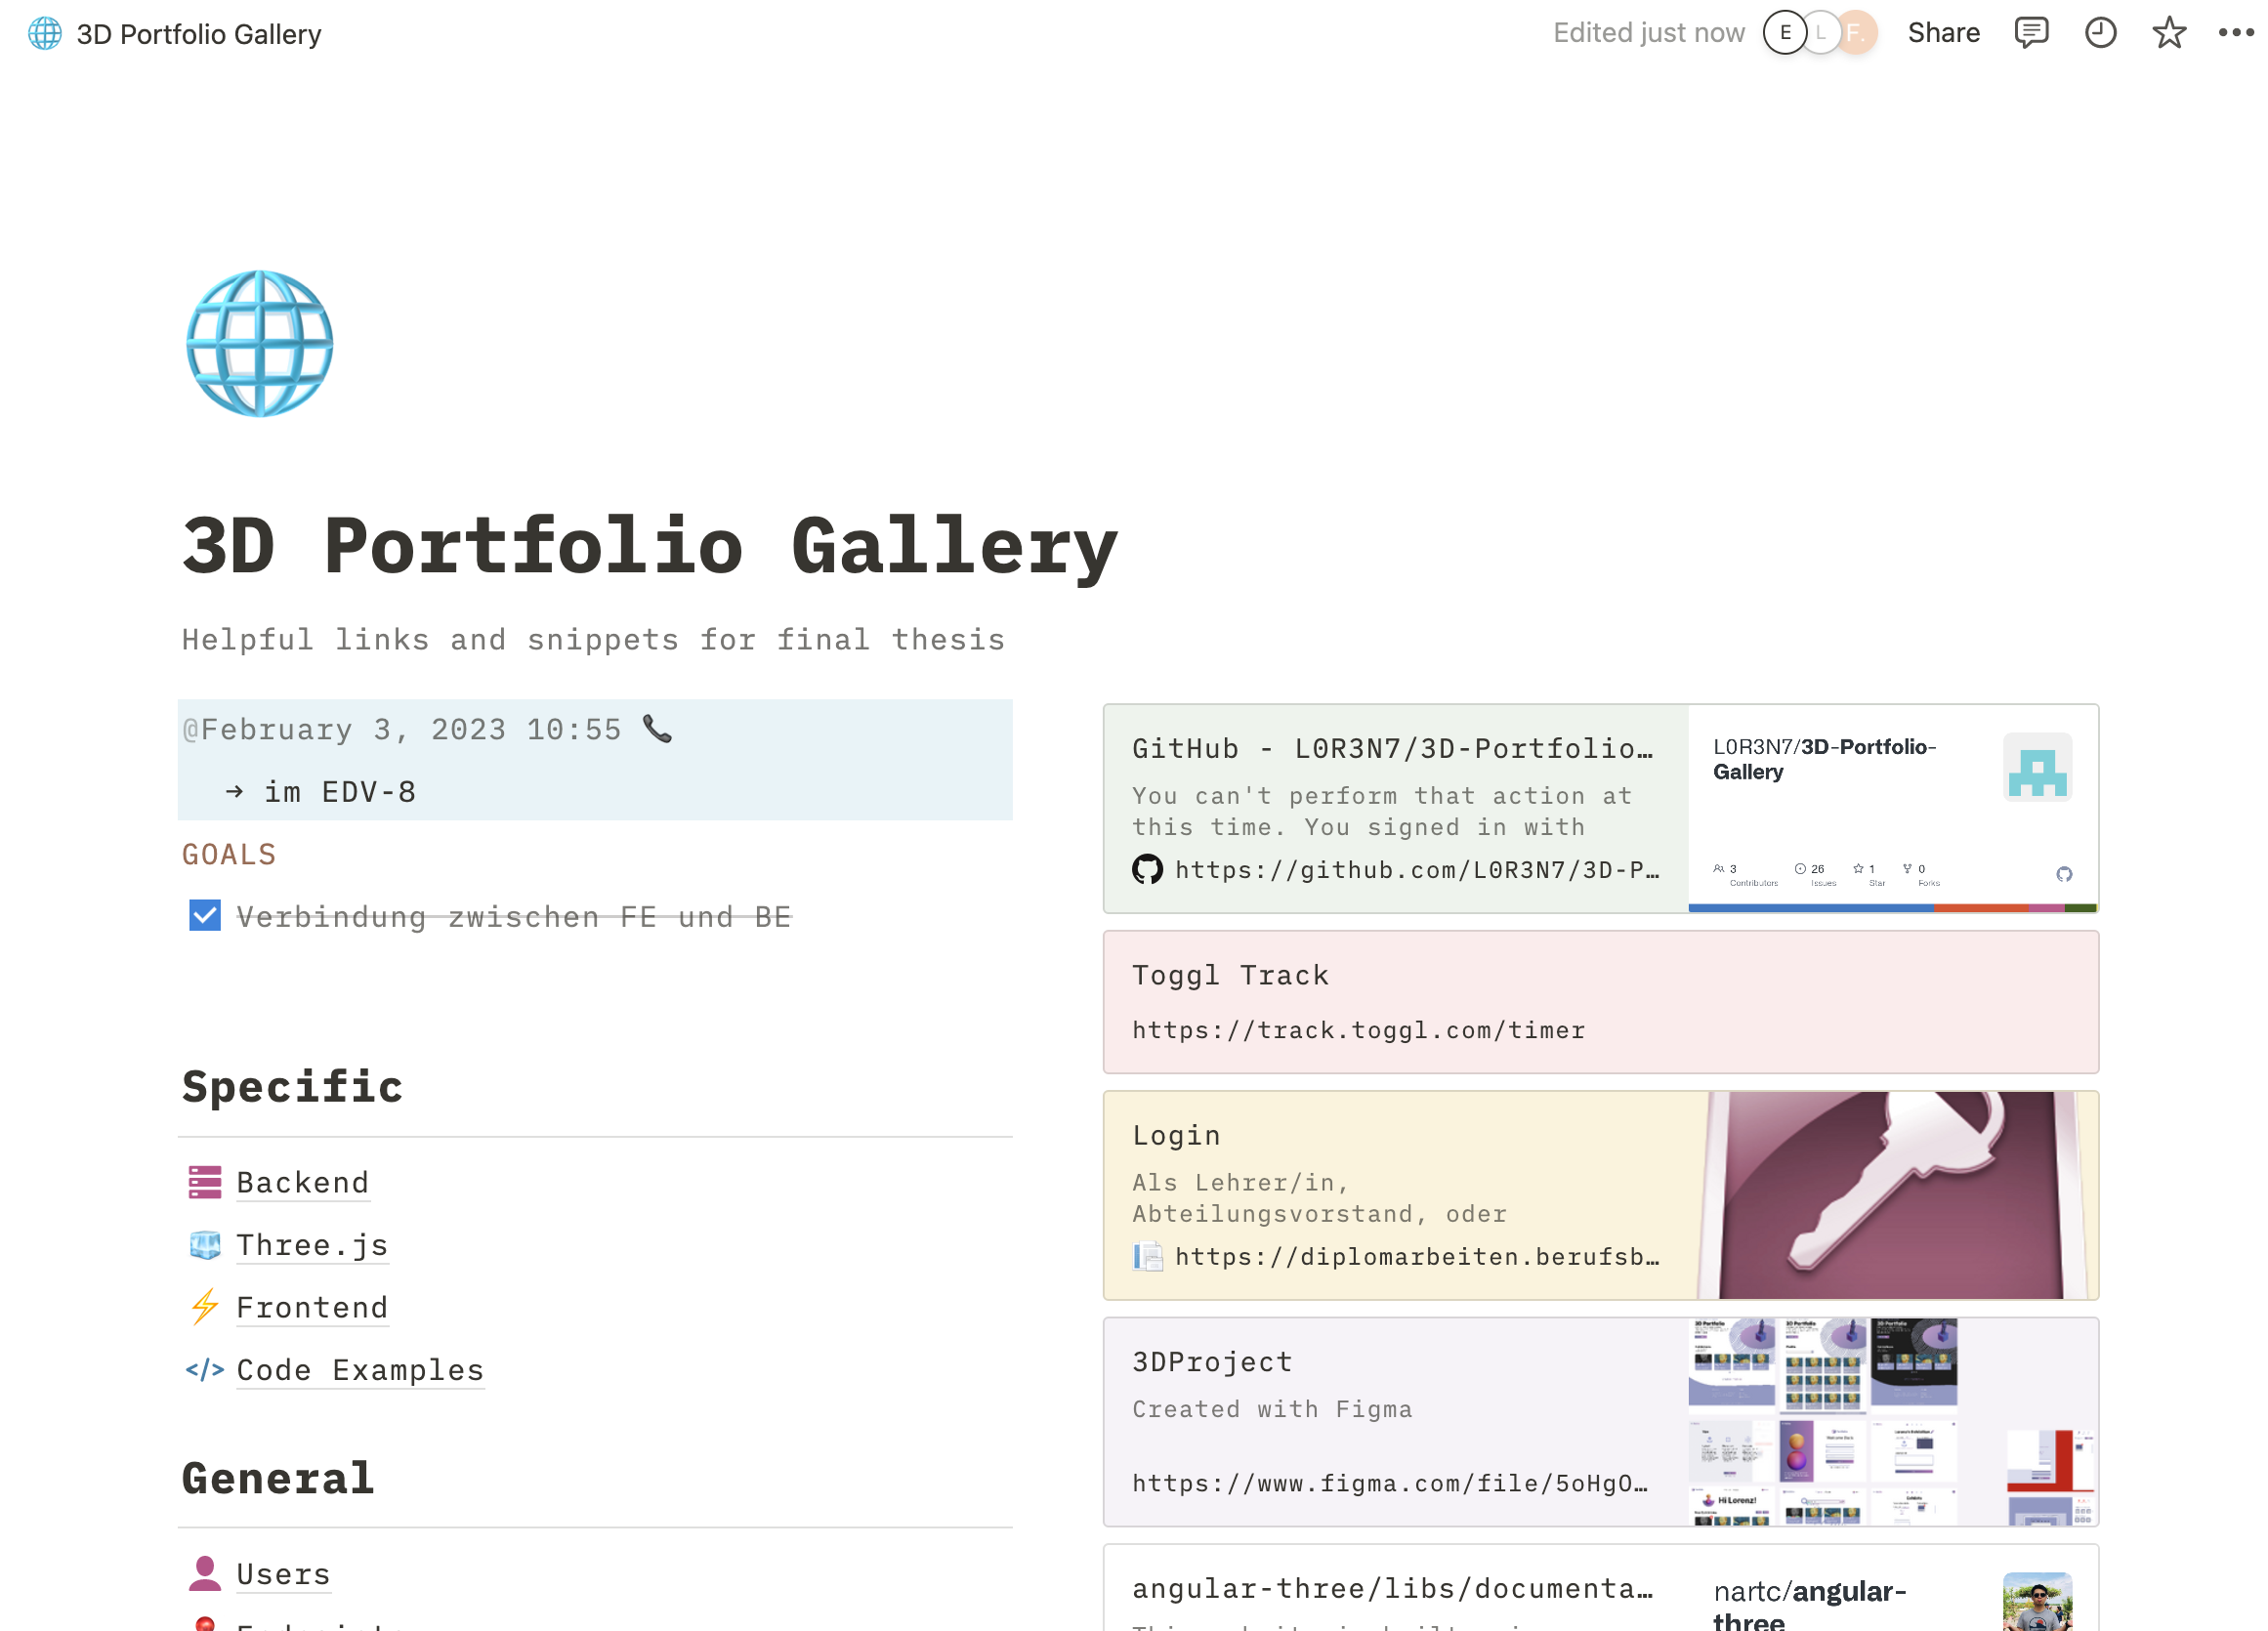
\includegraphics[scale=0.3]{pics/NotionPage.png}
  \caption{Notion Workspace der Diplomarbeit}
  \label{fig:tech:notion-page}
\end{figure}

\section{PlantUML}
PlantUML ist ein Tool, welches die Erstellung von \gls{uml}-Diagrammen vereinfacht. 
Das Ziel von \gls{uml} ist es, Tools zu liefern, um Systeme zu visualisieren.
\cite{UMLPaper}
Dafür gibt es verschiede Arten von \gls{uml}-Diagrammen, wie beispielsweise Objektdiagramme oder Sequenzdiagramme.
\cite{PlantUML}


Für diese Arbeit wurde ein \gls{erd} mit Krähenfußnotation, auch bekannt als Martin-Notation, verwendet.

\section{JSON Web Token}
JSON Web Token, oder \gls{jwt}, sind eine Methode, um Daten sicher zu Übertragen. 
Sie können über eine digitale Signatur besitzen, wie zum Beispiel eines RSA Schlüsselpaars, oder eines HMAC Algorythmus. 
In diesem Token ist es möglich Daten zu speichern, sowie eine \gls{ttl} festzulegen. 
Die Authentifizierung geschieht durch das Mitgeben des Tokens im Header. 
Jeder Token muss validiert werden, wodurch ihm eine Signatur hinzugefügt wird. 
Diese wird mittels den vorher gennaten Methoden umgesetzt. 
\cite{JWTAbout}

%\subsection{Deeper}
%Nicht mehr im Inhaltsverzeichnis.

%\subsubsection{Deepest}
%Vermeide mich.